\chapter*{Appendix}
\section{Unused plots}
\label{App:Plots}
\begin{figure}[H]
    \centering
    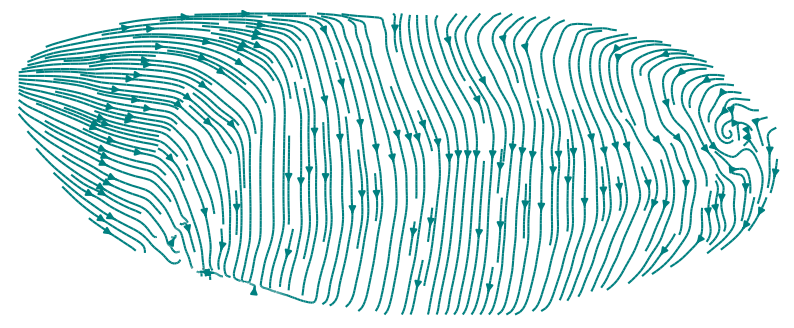
\includegraphics[width=1\linewidth]{chapters/Appendix/streamplot1.png}
\end{figure}
\begin{figure}[H]
    \centering
    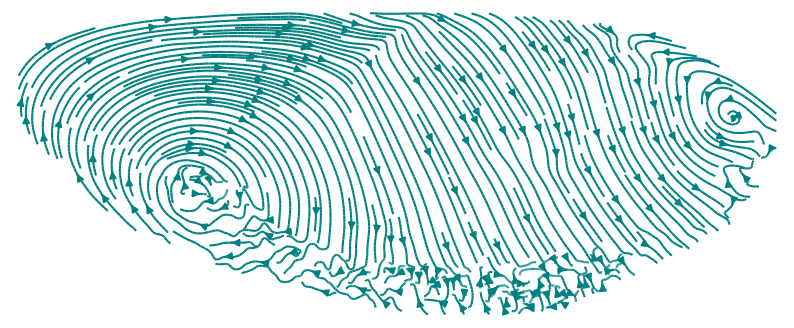
\includegraphics[width=1\linewidth]{chapters/Appendix/streamplot2.png}
    \caption{Cool but ultimately non-useful flow-field plots}
    \label{fig:enter-label}
\end{figure}

\begin{figure}[H]
    \centering
    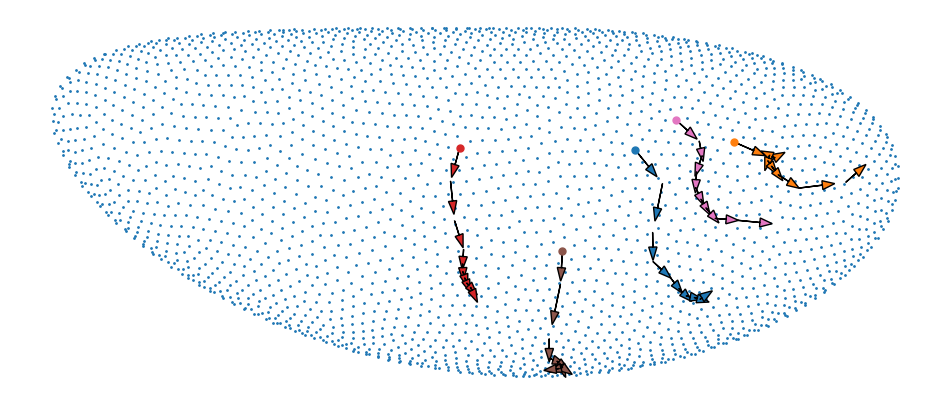
\includegraphics[width=1\linewidth]{chapters/Results/figures/movements.png}
    \caption{\todo{Remove some of the cells -- it's cluttered. Change color over time}}
    \label{fig:GBMovements}
\end{figure}

\begin{figure}[H]
    \centering
    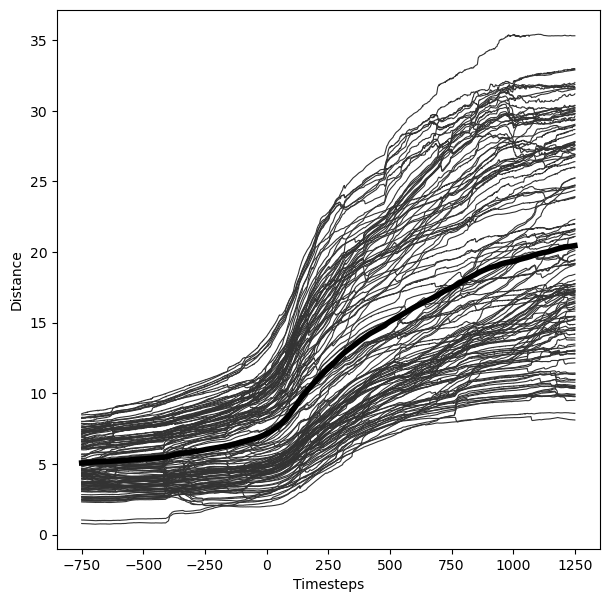
\includegraphics[width=1\linewidth]{chapters/Appendix/germbandMovementQuant.png}
    \caption{Horizontal-position of a line of germ-band cells, mirroring the analysis in  \url{https://www.ncbi.nlm.nih.gov/pmc/articles/PMC2801059/}}
    \label{fig:enter-label}
\end{figure}
\begin{figure}[H]
    \centering
    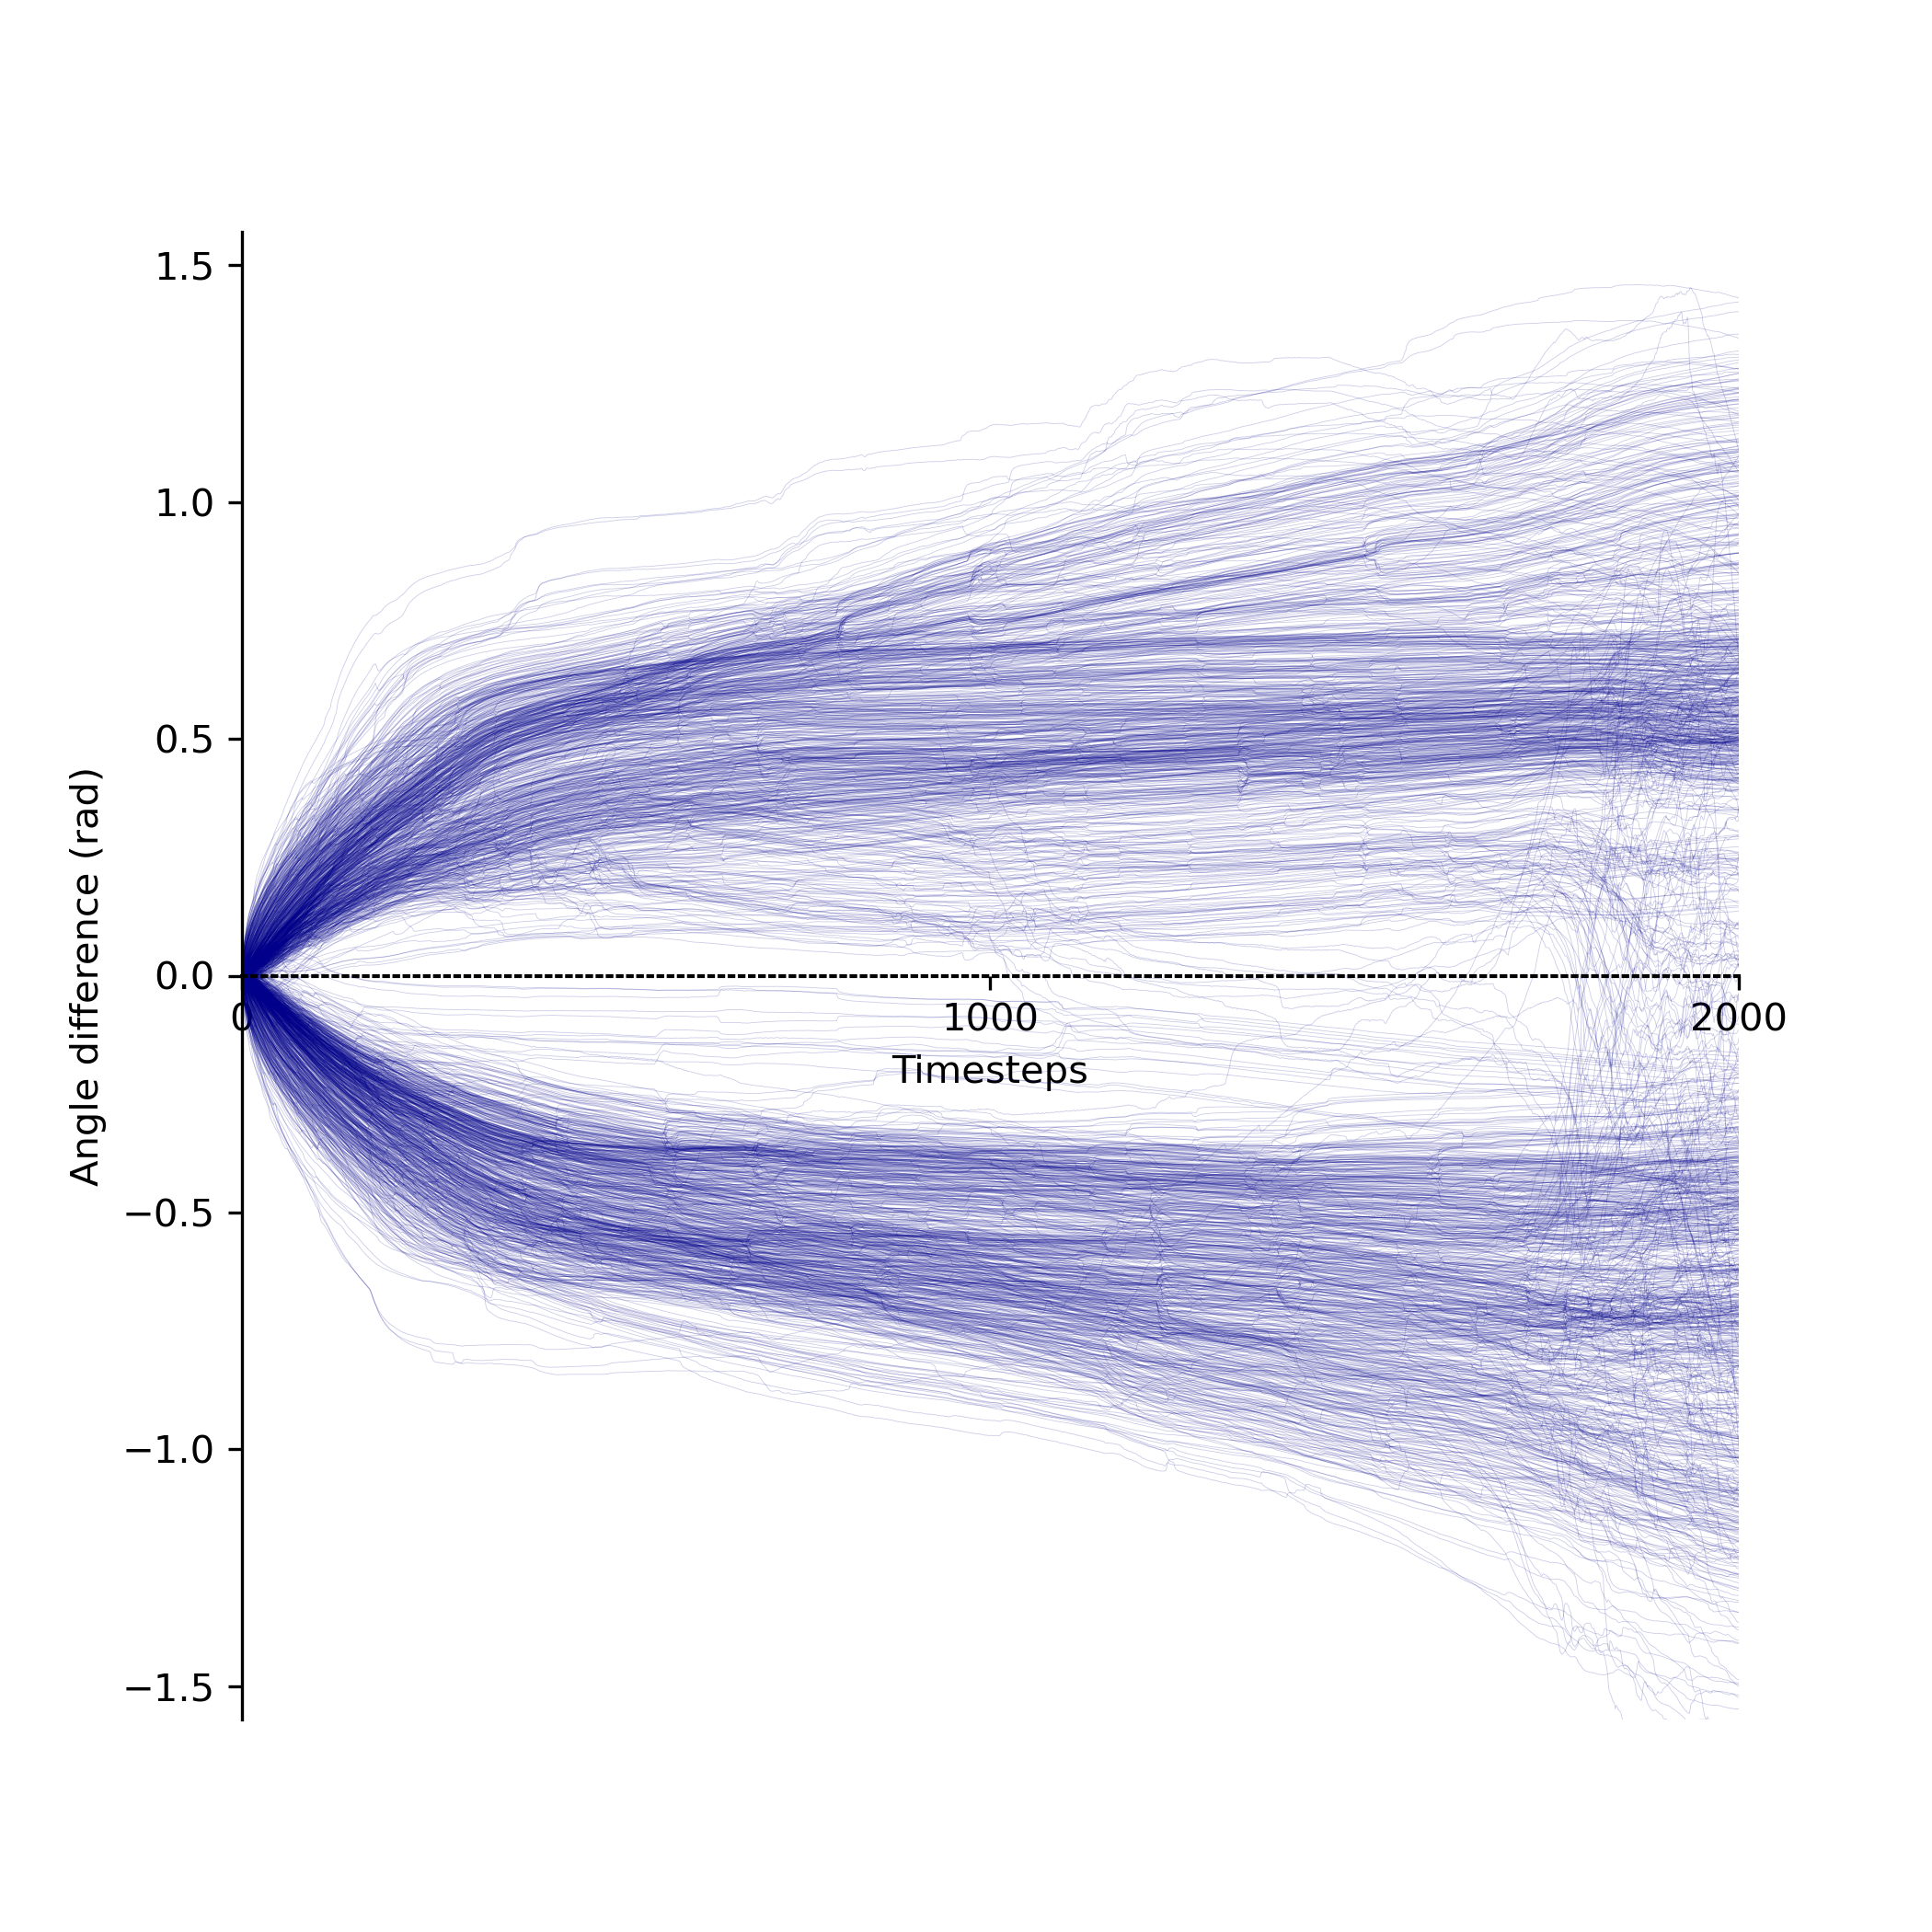
\includegraphics[width=1\linewidth]{chapters/Appendix/the_ring.png}
    \caption{Angle in cylindrical coordinates of germ-band. Mirroring \url{https://www.ncbi.nlm.nih.gov/pmc/articles/PMC2801059/}}
    \label{fig:enter-label}
\end{figure}
\section{Code details}
\label{App:Code}
\section{Additional Videos}
\label{App:videos}
\section{Sergei-analyses (tie into PCP)}
\label{App:Sergei}
\section{Green-Lagrange strain inference}
\label{App:Strain-Calculation}
Firstly transform into cylindrical coordinates.... \\
"A strain rate is the ratio of the change in length to the original length, divided by the time interval, with units of proportion (pp) per minute. The lines show the mean strain rates for all five embryos, and the ribbon width represents the average standard error within a data set. The timing of developmental landmarks is shown for the five embryos recorded"\cite{butler2009cell}
\section{Why our rosettes behave differntly }
\label{App:why-rosettes}
In our model, where the equilibrium distance is the same for every direction no matter the pressure exerted, getting a bimodality is predictable.
Every time a new pair 'touch' on the up-down axis, they release space for a pair above or below on the perpendicular axis. 


\section{We have not taking the following into account}
\subsection*{Cell shape change!}
\subsection*{Mitotic pressure in cephalic area}
\subsection*{Things that change over time}
\subsection*{Pressure-buckling of dorsal folds}
\subsection*{Pressure from yolk}
\section{Detailed morphogens}
\label{App:morphogens}

\begin{table}[H]
\begin{tabular}{lll}
 \begin{tabular}[c]{@{}l@{}}Genetically patterned \\ transcription factor proteins\end{tabular} & Location at gastrulation & Vital for development of \\ \hline
 Twist \& Snail                                                                                 & Ventral                  & Mesoderm                 \\
Huckebein \& Tailless                                                                          & Posterior                & Endoderm (Midgut)   \\

 Runt \& Even skipped & Germ Band & All of the above\\
Buttonhead \& Even skipped  & Cephalic furrow & Chephalic furrow\\

\end{tabular}
    \caption{The most important morphogens and their simplified reason of significance}
    \label{tab:morphogens}
\end{table}

\section*{Other efforts we have tried in vain}

